\documentclass[12pt, oneside]{article}   	% use "amsart" instead of "article" for AMSLaTeX format
\usepackage{geometry}                		% See geometry.pdf to learn the layout options. There are lots.
\geometry{letterpaper}                   		% ... or a4paper or a5paper or ... 
%\geometry{landscape}                		% Activate for rotated page geometry
%\usepackage[parfill]{parskip}    		% Activate to begin paragraphs with an empty line rather than an indent
\usepackage{graphicx}				% Use pdf, png, jpg, or eps§ with pdflatex; use eps in DVI mode
								% TeX will automatically convert eps --> pdf in pdflatex		
\usepackage{amssymb}
\usepackage{newcommand_yye}
\usepackage{hyperref} % super link

%SetFonts

%SetFonts


\title{Validation de $p_k$ sur un cercle}
\author{Yilin YE}
\date{02 juin 2023}							% Activate to display a given date or no date

\begin{document}
\maketitle


\sct{Près de centre, $r_0 = 0.1$}
On considère $p_k$ sur un cercle avec son rayon égal 1. 
On sait la densité de la mesure harmonique comme:
\eq{ \omega_q (\theta|r_0,\theta_0) = \frac{1}{2\pi R} \times \llc 1 + 2 \sum_{j=1}^\infty \llp \frac{r_0}{R} \rrp^j  \frac{\cos \lls j(\theta-\theta_0) \rrs}{1 + \frac{j}{qR}} \rrc \tlag{1}}
En pratique, on prend les positions initiales $(x_0,y_0) = (0.1,0.0)$, et donc $(r_0,\theta_0) = (0.1,0.0)$.


Comme ici il n'y a pas de segments, on peut tout simplement diviser le cercle en $N$ arcs identiques caractérisés par l'angle $\frac{2\pi}{N} (k-1) \le \theta < \frac{2\pi}{N} k$, avec $k = 1,2,3,...,N$, et définir
\eq{ \agn{
& p_k = \int_{\frac{2\pi}{N}(k-1)}^{\frac{2\pi}{N} k} \omega_q(\theta|r_0,\theta_0) d \theta \\
&= \invs{\pi R} \llc \frac{\pi}{N} + \sum_{j=1}^\infty \llp \frac{r_0}{R} \rrp^j  \frac{\sin \lls j \llp \frac{2\pi}{N} \cdot k -\theta_0 \rrp \rrs - \sin \lls j \llp \frac{2\pi}{N} \cdot (k-1) -\theta_0 \rrp \rrs}{\frac{1}{j} + \frac{1}{q R} } \rrc 
} \tlag{2} }


Numériquement, on prend $10^6$ particules, $j_\mrm{max}=10$, et $N = $ 60 ou 180. Voici les résultats analytiques (en rouge) et ceux numériques (en noire). Alors, on vérifie bien ces deux courbes.


\begin{center}
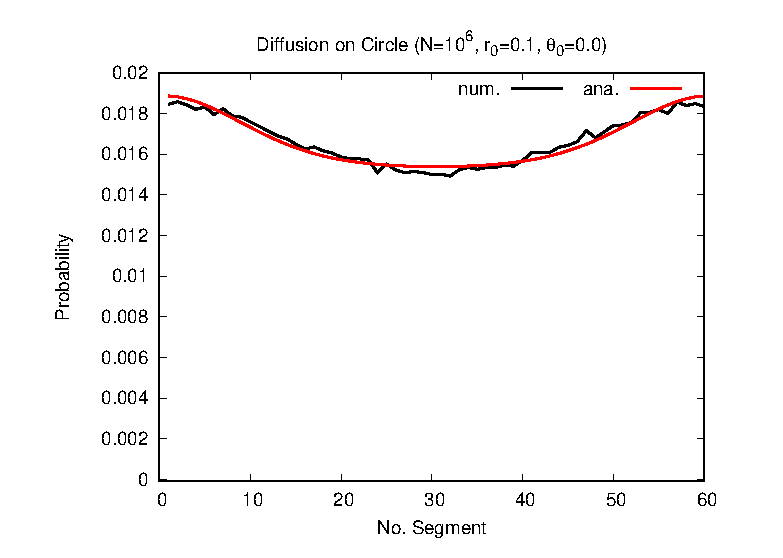
\includegraphics[width=0.48\linewidth]{pbb_cc_N60.eps}
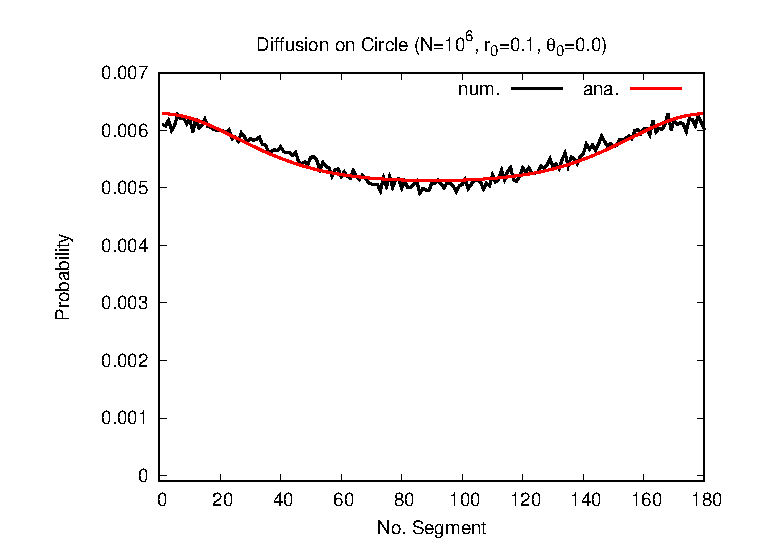
\includegraphics[width=0.48\linewidth]{pbb_cc_N180.eps}
\end{center}





\sct{Près de frontière, $r_0 = 0.9$}

Malheureusement, quand on fait la simulation près de frontière, i.e. $r_0 = 0.9$, on voit un résultat bizarre.
\begin{figure}[ht]
\centering
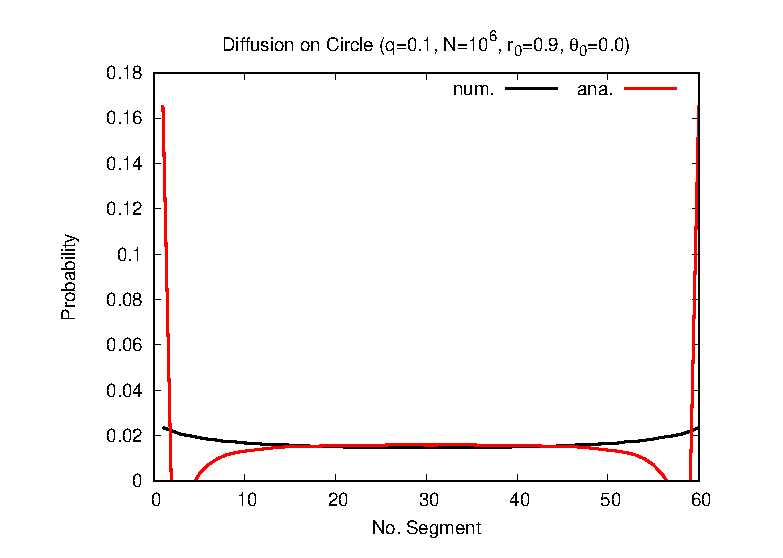
\includegraphics[width=0.9\linewidth]{res/sim-6/pbb_cc.eps}
\end{figure}

En effet, c'est pas possible d'obtenir la probabilité negative. Ainsi, on retourne l'équation \ref{1} et re-fait l'intégration
$$ \int_{\frac{2 \pi}{N} (k-1)}^{\frac{2 \pi}{N}k} \frac{2 \left(\frac{r_0}{R}\right)^j \cos (j (\theta -\theta_0))}{(2 \pi  R) \left(\frac{j}{q R}+1\right)} \md\theta = \frac{2 q}{\pi j (j + q R)} \left(\frac{r_0}{R}\right)^j \sin \left(\frac{\pi  j}{N}\right)  \cos \left(\frac{j (-2 \pi  k+N \theta_0+\pi )}{N}\right) $$
Et donc on récrit l'équation \ref{2} comme
\eq{ \agn{
& p_k = \int_{\frac{2\pi}{N}(k-1)}^{\frac{2\pi}{N} k} \omega_q(\theta|r_0,\theta_0) d \theta \\
&= \invs{N R} + \sum_{j=1}^\infty  \frac{2 q}{\pi j (j + q R)} \left(\frac{r_0}{R}\right)^j \sin \left(\frac{\pi  j}{N}\right)  \cos \left(\frac{j (-2 \pi  k+N \theta_0+\pi )}{N}\right)
} \tlag{3} }


Ensuite, on refait les simulations avec des résultats analytiques par l'équation \ref{3}. Ici, les positions initiales sont près de frontière, i.e. $r_0 = 0.9$, et on prend la réactivité comme $q = 10, 1, 0.1$. Comme vu, on vérifie bien ces résultats.


\begin{center}
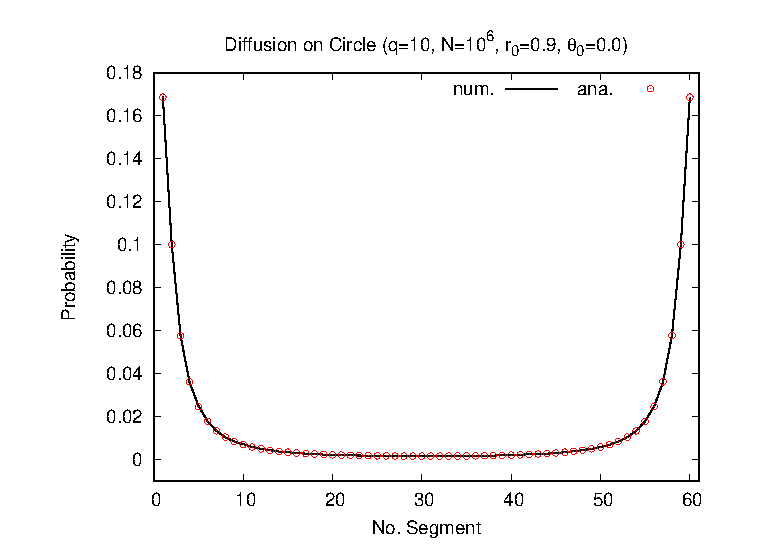
\includegraphics[width=0.9\linewidth]{res/sim-7/pbb_cc.eps}
\end{center}
\begin{center}
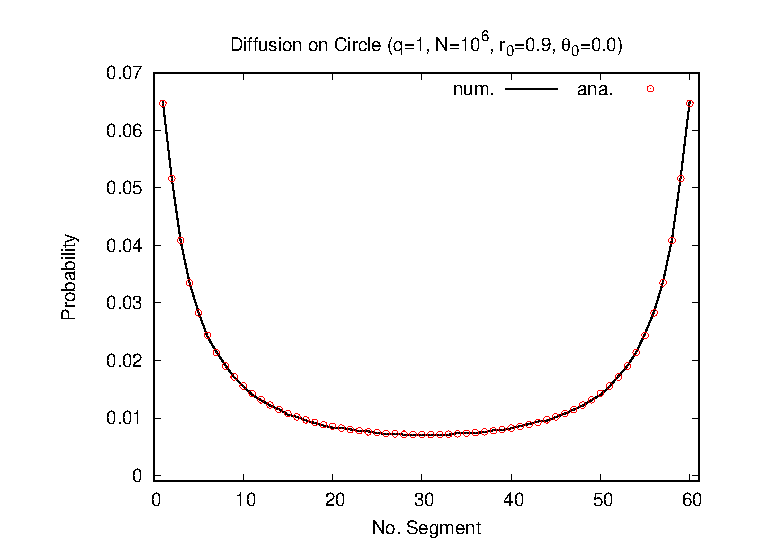
\includegraphics[width=0.9\linewidth]{res/sim-8/pbb_cc.eps}
\end{center}
\begin{center}
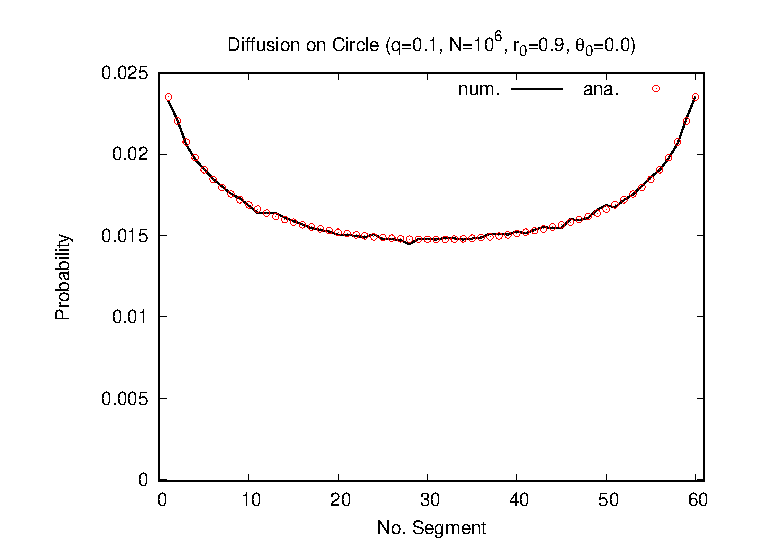
\includegraphics[width=0.9\linewidth]{res/sim-9/pbb_cc.eps}
\end{center}







\end{document}  